% ..............................................................................
% Demo of the fau-beamer template.
%
% Copyright 2022 by Tim Roith <tim.roith@fau.de>
%
% This program can be redistributed and/or modified under the terms
% of the GNU Public License, version 2.
%
% ------------------------------------------------------------------------------

% ------------------------------------------------------------------------------
\section{Randomness and Non-Randomness}
% ..............................................................................
% Source of randomness
\subsection{Source of randomness}
\begin{frame}[t]{Source of randomness}{The library metapher}
	\begin{itemize}
		
		\item \textbf{A seeming conflict}
		\begin{itemize}
			\item \textit{statistical methods ... operate on random samples}
			\item \textit{very little (in language) is left to chance}
		\end{itemize}
		\bigbreak
			
		\item \textbf{The library metapher}
		\begin{itemize}
			\item \textit{... there is nothing random about the text in the library: every senetence was produced for some specific purpose.}
			\item \textit{The selection of a particular corpus} - \textit{picking an arbitrary book from one of the shelves}
			\item \textit{It is this choice which introduces an element of randomness into corpus frequency data.}
		\end{itemize}
		\bigbreak
		
		\item \textbf{Why randomness?}
		\begin{itemize}
			\item Statistical inference: Representativeness to (sub)language as a whole
		\end{itemize}
		
	\end{itemize}
\end{frame}

\begin{frame}{Source of randomness}{Illustrated in the procedures}
	\begin{figure}
		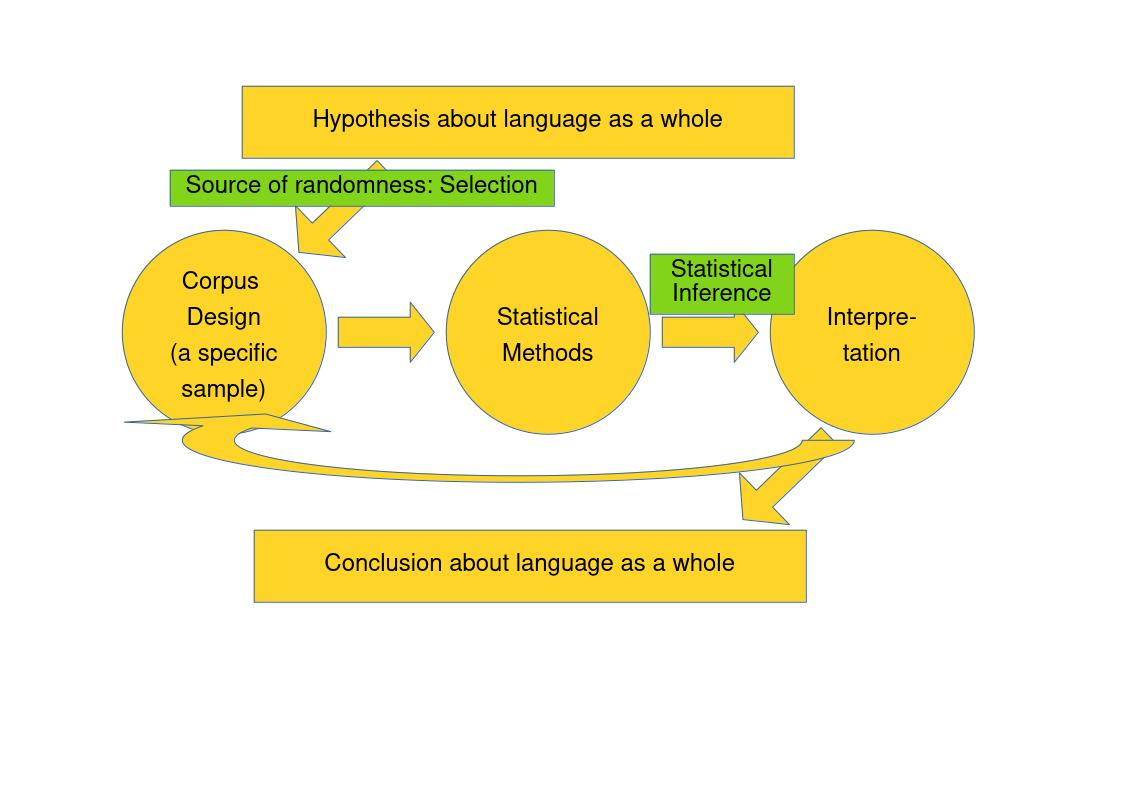
\includegraphics[width=.7\textwidth]{Figures/Randomness.jpg}
		\caption{Source of randomness}
	\end{figure}
\end{frame}


% Sources of non-randomness
\subsection{Sources of non-randomness}
\begin{frame}[t]{Sources of non-randomness}{Still not (completely) random?}
	
	\begin{itemize}
		\item \textbf{\textit{Balanced} samples}
		\begin{itemize}
			\item \textbf{External} source of non-randomness
			\item An issue of subjective language interpretation
		\end{itemize}
		\bigbreak
		
		\item \textbf{The unit of sampling} vs. \textbf{the unit of measurement}
		\begin{itemize}
			\item \textbf{Internal} source of non-randomness
			\item Clustering effect: \textit{a tendency to lump together}
			\item Language is NOT a bag of random words
		\end{itemize}
	\end{itemize}

\end{frame}

\begin{frame}{An evidence of internal non-randomness}{Underestimated variation}
	\begin{figure}
		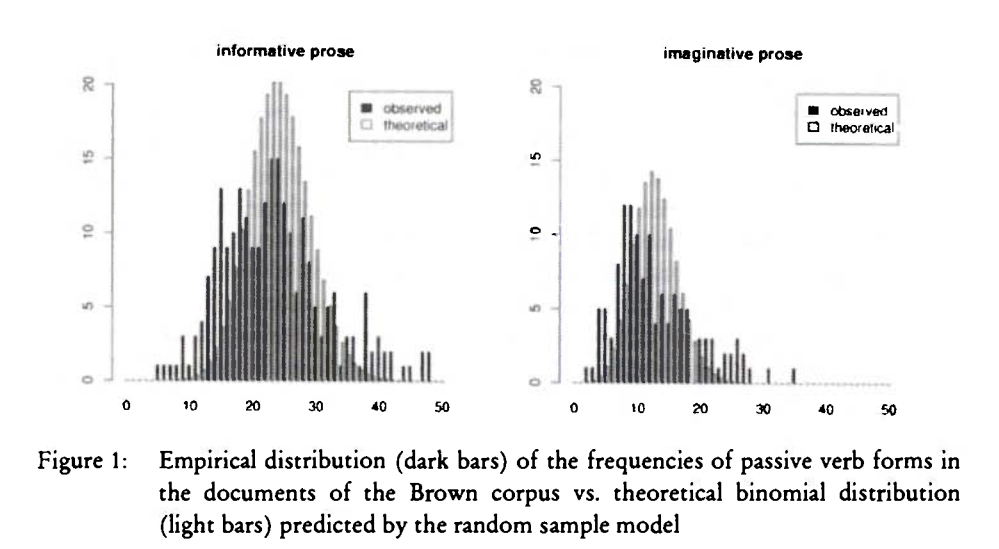
\includegraphics[width=.7\textwidth]{Figures/Distribution.png}
	\end{figure}
\end{frame}


